\documentclass[crop,tikz]{standalone}% 'crop' is the default for v1.0, before it was 'preview'
\usepackage{tikz,calc,pgfplots}
\usetikzlibrary{calc,patterns}
\begin{document}
	



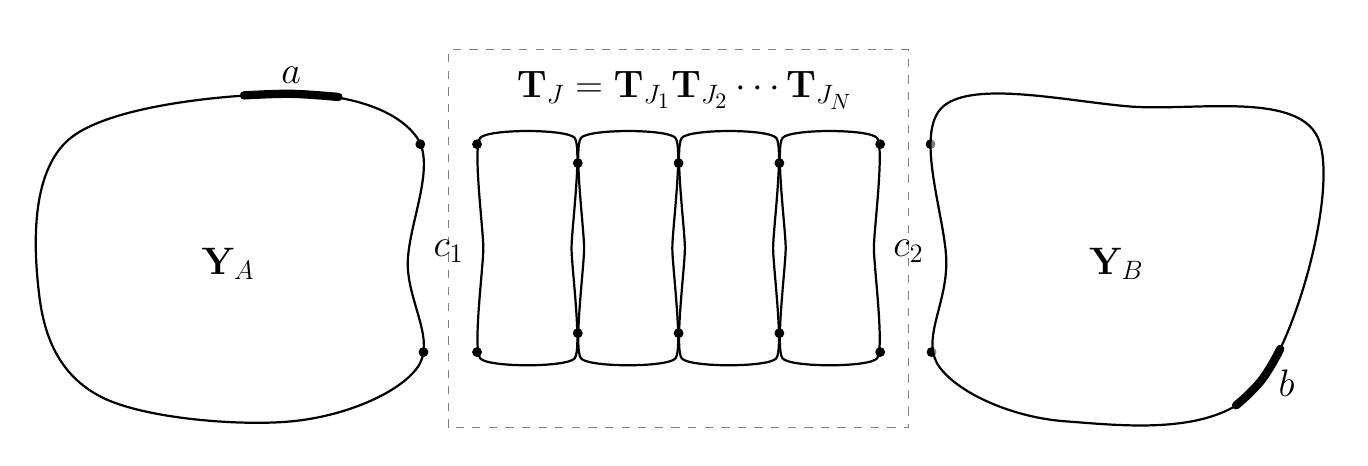
\begin{tikzpicture}[scale=0.8, every node/.style={transform shape}]
	
	\draw[draw=gray,dashed] (6.5,-0.1) rectangle ++(7.3,6);
		\node[outer sep=0pt,thick] at (10.25,5.25) [minimum width=1.5cm, minimum height=1.5cm] {\LARGE${\mathbf{T}_J}= \mathbf{T}_{J_1}\mathbf{T}_{J_2}\cdots \mathbf{T}_{J_N}$};
	
	
	\draw [thick,fill=white,fill opacity=0.5]  plot[smooth cycle, tension=.6] coordinates {(0,2) (0.5,4.5) (4,5.2) (6,4.5)  (5.85,2.5) (6,0.85) (4,0)  (1,0.38) };
	
	\node[outer sep=0pt,thick] at (3,2.5) [minimum width=1.5cm, minimum height=1.5cm] {\LARGE${\mathbf{Y}_A}$};
	
	\draw [line width=3pt,black,cap=round]  plot[smooth, tension=.6] coordinates { (3.25,5.175) (4,5.2) (4.75,5.15) };  
	\node[outer sep=0pt,thick] at (4,5.5) [minimum width=1.5cm, minimum height=1.5cm] {\LARGE$a$};
	
	\node[mark size=2pt,black] at (6.1,1.1) {\pgfuseplotmark{*}};
	\node[mark size=2pt,black] at (6.05,4.4) {\pgfuseplotmark{*}};	
	
	\node[outer sep=0pt,thick] at (6.5,2.7) [] {\LARGE$c_1$};
	
	\begin{scope}[xshift =7cm]
	\draw [thick,fill=white,fill opacity=0.5]  plot[smooth cycle, tension=.3] coordinates {(0,1)  (0.05,2.75) (0,4.5) (1.5,4.5)  (1.45,2.75) (1.5,1)  };
		\node[mark size=2pt,black] at (-0.05,1.1) {\pgfuseplotmark{*}};
		\node[mark size=2pt,black] at (-0.05,4.4) {\pgfuseplotmark{*}};	
	\end{scope}
	
	\begin{scope}[xshift = 8.6cm]
		\draw [thick,fill=white,fill opacity=0.5]  plot[smooth cycle, tension=.3] coordinates {(0,1)  (0.05,2.75) (0,4.5) (1.5,4.5)  (1.45,2.75) (1.5,1)  };
		\node[mark size=2pt,black] at (-0.05,1.4) {\pgfuseplotmark{*}};
		\node[mark size=2pt,black] at (-0.05,4.1) {\pgfuseplotmark{*}};	
	\end{scope}
	
	\begin{scope}[xshift = 10.2cm]
		\draw [thick,fill=white,fill opacity=0.5]  plot[smooth cycle, tension=.3] coordinates {(0,1)  (0.05,2.75) (0,4.5) (1.5,4.5)  (1.45,2.75) (1.5,1)  };
		\node[mark size=2pt,black] at (-0.05,1.4) {\pgfuseplotmark{*}};
		\node[mark size=2pt,black] at (-0.05,4.1) {\pgfuseplotmark{*}};	
	\end{scope}
		
	\begin{scope}[xshift = 11.8cm]
		\draw [thick,fill=white,fill opacity=0.5]  plot[smooth cycle, tension=.3] coordinates {(0,1)  (0.05,2.75) (0,4.5) (1.5,4.5)  (1.45,2.75) (1.5,1)  };
		\node[mark size=2pt,black] at (-0.05,1.4) {\pgfuseplotmark{*}};
		\node[mark size=2pt,black] at (-0.05,4.1) {\pgfuseplotmark{*}};	
		
		\node[mark size=2pt,black] at (1.55,1.1) {\pgfuseplotmark{*}};
		\node[mark size=2pt,black] at (1.55,4.4) {\pgfuseplotmark{*}};	
	\end{scope}
	
	\begin{scope}[xshift = 14.3cm]
		
		\node[mark size=2pt,black] at (-0.135,1.1) {\pgfuseplotmark{*}};

		
		\node[mark size=2pt,black] at (-0.15,4.4) {\pgfuseplotmark{*}};

		\node[outer sep=0pt,thick] at (-0.5,2.7) [] {\LARGE$c_2$};
		
		\draw [thick,fill=white,fill opacity=0.5]  plot[smooth cycle, tension=.6] coordinates {(0,0.85) (0.1,2.5) (0.05,5) (3,5) (6,4.5) (5,0.5) (2,0) };
		\node[outer sep=0pt,thick] at (2.8,2.5) [minimum width=1.5cm, minimum height=1.5cm] {\LARGE${\mathbf{Y}_B}$};
		
		
		\draw [line width=3pt,black,cap=round]  plot[smooth, tension=.8] coordinates { (4.7,0.255) (5.1,0.65)  (5.4,1.15)}; 
		
		\node[outer sep=0pt,thick] at (5.5,0.6) [minimum width=1.5cm, minimum height=1.5cm] {\LARGE$b$};
		
	\end{scope}
\end{tikzpicture}
\end{document}
